\chapter{Methodology}
\label{ch:methodology}

\begin{marginfigure}
    \centering
    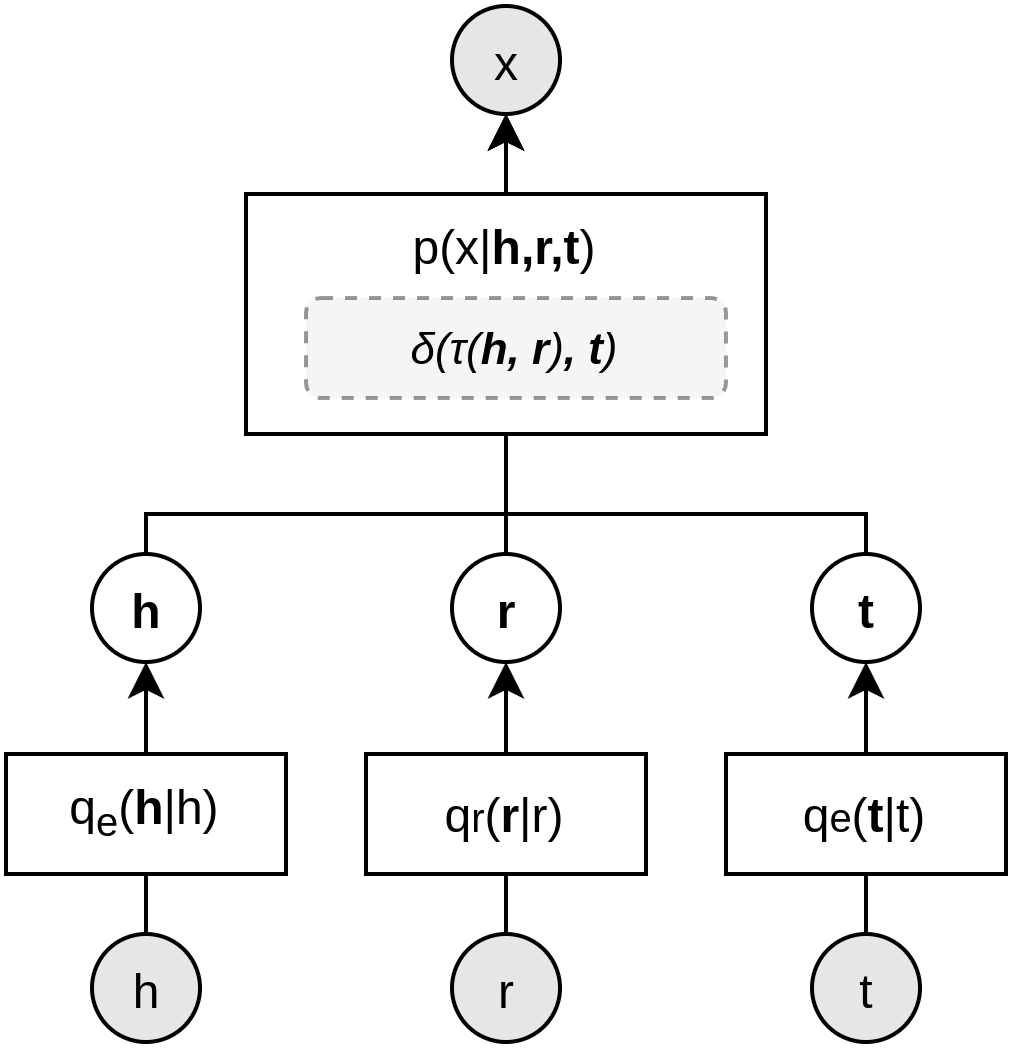
\includegraphics[width=1.\linewidth]{figures/base.png}
    \caption[Example of model diagram.]{Example of model diagram. The circles represent random variables, gray circles are observed, white circles unobserved. The boxes and arrows represent modeling decisions, for example here we model the probability of $x$ as being dependent on the embeddings $\vec{h}, \vec{r}, \vec{t}$. }
    %The gray rectangle containing $\sigma(\delta(\tau(\vec{h},\vec{r}),\vec{t}))$ gives specific information on the way that the distribution $p(x|\vec{h},\vec{r},\vec{t})$ is parameterized.}
    \label{fig:example_model_diagram}
\end{marginfigure}

This chapter describes and motivates the various ways in which we incorporate type information.
Some methods are original designs, for others we take inspiration from previous work.
The methods are described using both the notation introduced in the previous chapters, and using diagrams depicting the structure of the model (for example, a typical geometric model is depicted in Figure \ref{fig:example_model_diagram}).

\section{Objectives}\label{sec:method:objectives}%
The main objective is to answer the research question as given in Chapter \ref{ch:introduction}:
\begin{quote}
    \textit{(\textbf{RQ1})}
To what extent can type-information improve link-prediction performance? And,
\textit{(\textbf{RQ2})}
what method of incorporating the type-information is most effective?
\end{quote}
%
However, while answering our research question it might be useful to keep in mind some additional objectives. To maximize the utility of our investigations, we will keep in mind three secondary objectives, which are described below. Note that our methodology is not directly aimed at addressing these, but all things being equal, will try to nonetheless.

\subsection{Link Prediction as a proxy for general purpose embedding}
Knowledge Graph Embeddings may be used for a variety of downstream tasks such as: relation extraction, question answering, or recommender systems \mycitep{wang_knowledge_2017}. 
%Often the ability to predict links is still used as the primary objective during training. 
%This ability is regarded as indicative of
It will be useful to keep in mind how the different ways we incorporate type-information will affect these kinds of use cases.


\subsection{Anonymous entity embedding}
Using type information can allow us to embed entities that were not seen during training, as long as we know its type. 
%
To obtain such embeddings we need to model our embeddings as being conditioned on the types of the entity, i.e. $\vec{E}_i | C_{i,s}\!=\!c_{i,s}$.
Of particular interest is any model that accomplishes this without giving up the possibility of learning a specific embedding for the entities we do see during training.


% \subsection{Modeling uncertainty}
% Modeling the embeddings as probabilistic rather than point estimates (for example, like \mycite{he_learning_2015}) might be beneficial when it comes to incorporating type-information in the embeddings. For example, when learning embeddings for types using a point estimate to model a type, it seems we are at best learning a `prototypical' example of that type. With a distribution the variance can be tuned such that the probability mass covers all the space that the entities of that type exist in.


% An obvious way to improve upon KG2E is by using a type of normalizing flow such as Inverse Autoregressive Flow\cite{kingma_improved_2016}.

% One interesting avenue this method would open, is the ability to create a model where we first get $\vec{h}|h$, $\vec{r}|r$, $\vec{t}|t$ but then also have an additional posterior $\vec{h'},\vec{r'},\vec{t'}|\vec{h},\vec{r},\vec{t}$ such that the embeddings can be adapted by letting information flow between the different triple components. 
% %
% Of course you could just parameterize an approximate posterior $q(\vec{h'},\vec{r'},\vec{t'}|{h},{r},{t})$ from the beginning. But the downside of this is that we no longer have access to independent entity embeddings at all, only contextualized embeddings that are triple-specific.



\section{Using types to estimate prior probability of links}
\label{sec:method_type_linkprior}
%
The first method to be included in our experiments is the type-based prior introduced by \citeauthor{ma2017transt} in their paper on TransT (described in Section \ref{sec:transt}). 
It gives us an estimation of $p(h|r,t)$, $p(r|h,t)$, and $p(t|h,r)$.
It can easily be used in combination with any model to re-weight the scores assigned to each triple.
When used with a model that gives the likelihood of a triple, we can use the priors to get  approximated posteriors $p(h|r,t,x)$, $p(r|h,t,x)$, and $p(t|h,r,x)$.

By directly influencing the prediction for links, this approach is aimed at solving the primary objective. It does not address either of the additional objectives.

\paragraph{}\noindent
We do not include all configurations of TransT that \citeauthor{ma2017transt} propose. They distinguish between the configurations `type information', `multiple vectors' and `multiple+type'. In the first configuration the type-based prior is used to reweigh the scores as described above.
The second configurations refers to the representation of entities by multiple vectors. The number of vectors to be learned for each entity is based on the available type information (see Section \ref{sec:transt}). The last configuration combines the first two.
We include only the `type information' configuration, because any performance gain of the other configurations cannot easily be attributed to use of type-information, since it could also be attributed to the increase in the number of parameters.


\subsection{Type-linkprior only}
%
This method evaluates the type-based prior on its own.
We use only the score given by the prior to rank which triples are most likely to exist.
This gives us an indication of how informative the prior is, as well as a way to compare the datasets on the relative richness of their type information.
This configuration was not included in the experiments of \citeauthor{ma2017transt}.


\subsection{Type-linkprior+ScoringModel}
%
This method combines an existing ScoringModel, i.e. a model that already scores each triple, with the type-based prior. The final scores are those assigned by the ScoringModel multiplied by the estimated prior probability.
When the ScoringModel is TransE we obtain the configuration from which TransT derives its name.
This method is equivalent to \citeauthor{ma2017transt}'s `type information' configuration.


\section{Using types to construct the entity-embeddings}
%
Another way to use type information is to let each entity's set of types influence what the embedding of those entities will be. We experiment with three different kinds of embedders each with their own way of letting the types influence the entity-embeddings.
This type of model is displayed in Figure \ref{fig:type_for_entity_embeddings}.

\begin{marginfigure}
    \centering
    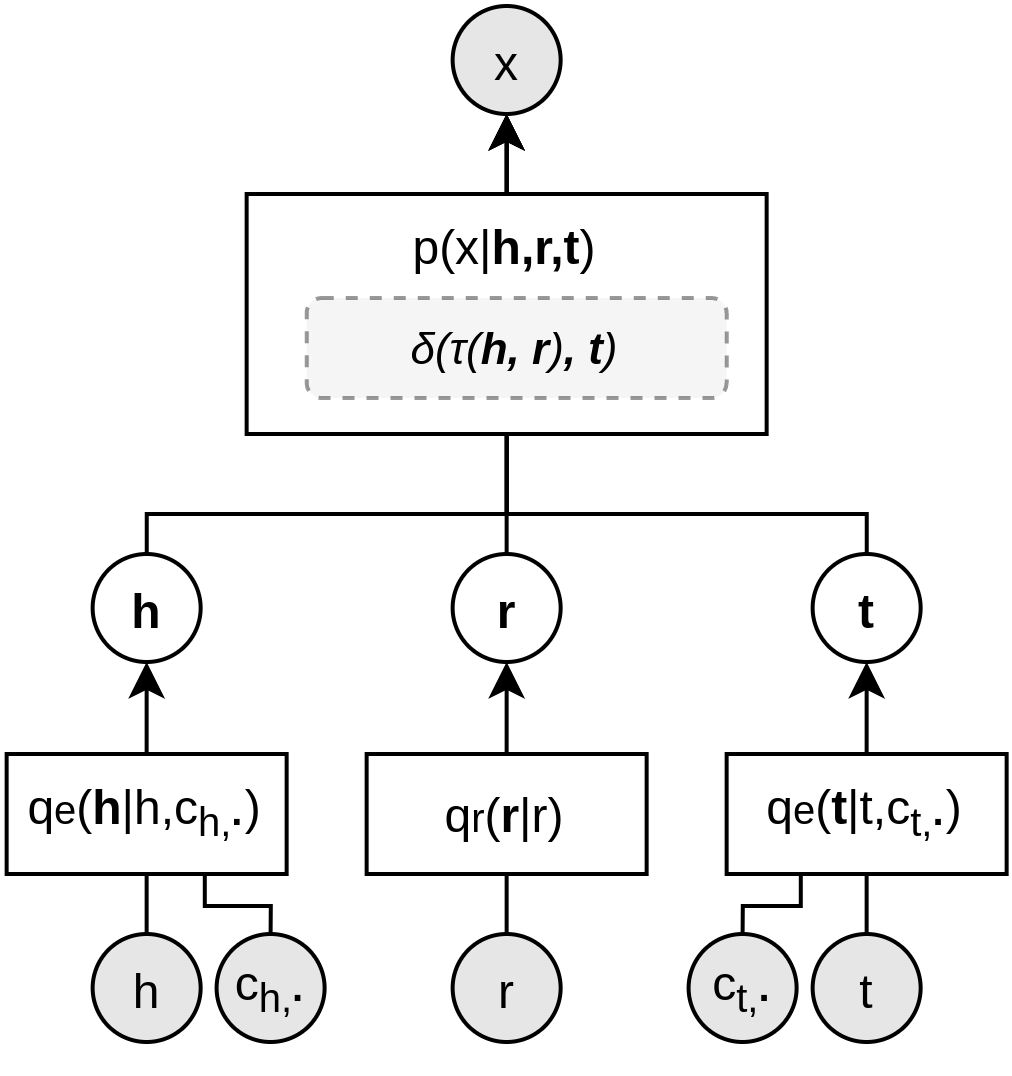
\includegraphics[width=\linewidth]{figures/type-embed.png}
    \caption[Model diagram with types for entity-embeddings.]{Diagram of model that utilizes types to construct entity-embeddings. }
    \label{fig:type_for_entity_embeddings}
\end{marginfigure}

% TYPE-MEAN
\subsection{Type-mean embedder}\label{sec:methods:type_mean}
This embedder is perhaps the simplest way of creating an entity's embedding from its types. Its main purpose is to serve as a baseline. 
%, showing what kind of performance is possible by including type-information in the entity-embeddings.
It learns embeddings for the types, and models an entity's embedding as the average of that entity's type embeddings, i.e.:
%\marginnote[2em]{We use $c_{i,\cdot}^+$ as short for $C_{i,\cdot} = True$.}
\begin{align}
    & \vec{C}_{s} | \theta_{s} && \simpnt \theta_{s} \\
%
%    & \vec{E}_i | C_{i,s} = c_{i,s} && = \underset{c_{i,s}}{\mathbb{E}} \left[ \vec{c}_s \right]
%    & \vec{E}_i | c_{i,1}^+, c_{i,2}^+, \dots, c_{i,Z}^+ && = \frac{1}{Z} \sum_{z=1}^{Z} \,\vec{c}_z
    & \vec{E}_i | c_{i,1}, c_{i,2}, \dots, c_{i,S} && 
    = \frac{\sum_{c_{i,z}} \vec{c}_z}{\sum_{c_{i,z}} 1} 
\end{align}
where $\theta_{s}$ are the model parameters that provide the point estimate for the $s$-th type's embedding.

\paragraph{Variant: adding entity offset embeddings.}
This variant learns an additional vector for each entity that we add to the mean of the type-vectors.
\begin{align}
    & \vec{E}_i | \epsilon_i, c_{i,1}, c_{i,2}, \dots, c_{i,S} && 
    = \frac{\sum_{c_{i,z}} \vec{c}_z}{\sum_{c_{i,z}} 1} + \epsilon_i
\end{align}
%
This addition could allow for more accurate embeddings for the entities, since two entities with the same types can now be specialized. 

This method could also be able to satisfy one of our secondary objectives. Specifically if the entity-offset is randomly dropped-out for some batches during training, it could allow us to embed both seen and unseen entities. Unseen entities are embedded by forgoing the entity-specific offset.
%
Furthermore the inclusion of the type-information in the entity-embeddings themselves may benefit downstream tasks.

% TYPE-ATTENTIVE
\subsection{Type-attentive embedder}
\begin{marginfigure}%[3.5cm]
    \centering
    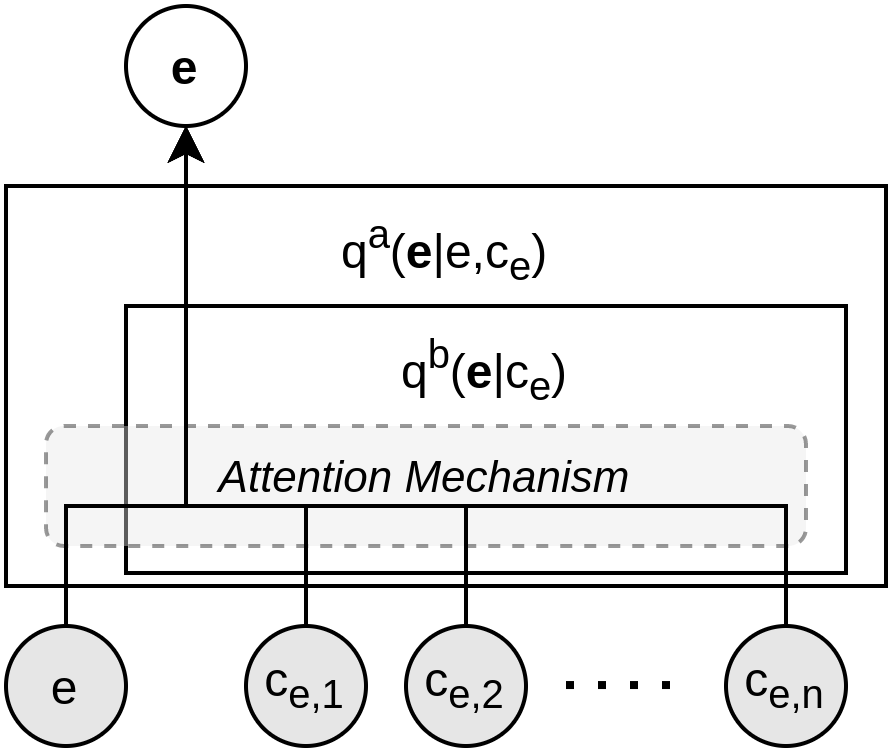
\includegraphics[width=\linewidth]{figures/type-attentive.png}
    \caption[Diagram of the type-attentive embedder.]{Diagram of the type-attentive embedder, depicting the two variants $q^a$ which includes the entity $e$ in the keys and values, and $q^b$ which does not. }
    \label{fig:type_attn_embed}
\end{marginfigure}

This embedder improves upon the type-mean embedder by learning to weight the type-embeddings differently for each entity. We do so with an attention mechanism:
\begin{align}
    & {q}_i             && =        ( \epsilon_i )^\top \\
    & {k}_i = {v}_i     && =        ( \theta_s | \mathcal{C}_{i,s})^\top \\
    & \vec{E}_i         && \simpnt  \mathrm{attn}(q_i, k_i, v_i)
\end{align}
where $\epsilon_i$ and $\theta_s$ are entity- and type-specific model parameters respectively.

\paragraph{Variant: adding the entity-vector to the keys and values.}
In this variant we allow the entity-vector to be included in the weighted average.
\begin{align}
    & {k}_i = {v}_i     && =        ( \epsilon_i ; \theta_s | c_{i,s})^\top 
\end{align}
This variant allows further specialization for each entity.

\paragraph{Mutual information loss.}
% hjelm_learning_2018
To encourage the inclusion of type information in the final entity-embeddings, we introduce an additional optimization objective. Taking inspiration from \mycite{hjelm_learning_2018}, we employ a mutual information based secondary objective.


%This idea is depicted in a diagram in Figure \ref{fig:type_attn_embed}. 

%\subsection{Idea}
%\begin{itemize}
    %\item Learn embeddings for entity-classes, as well as entities to get: $p(\vec{h}|c_h)$, $p(\vec{t}|c_t)$ and $p(\vec{h}|h)$, $p(\vec{t}|t)$. 
    %\item Combine those embeddings in an attention mechanism to also parameterize $p(\vec{h}|h,c_h)$ and $p(\vec{t}|t,c_t)$.
    %\item To meet requirement \ref{req:class-latent}, we would need to use $p(\vec{h}|c_h)$, $p(\vec{t}|c_t)$ to predict $x$ (some of the time) as an additional loss. 
    %\item Attention mechanism: 
    %    \begin{itemize}
    %        \item 1-N, keys = $\{ \vec{e} \}$, queries = values = $\{ \vec{e}, \vec{c}_{e,1}, %\dots, \vec{c}_{e,n} \}$ 
    %        \item $f_v(x) = x$; $f_q(x) = f_k(x) =  (x)$; \\ $out = \sum (f_k(x) \cdot f_q(x)) * %f_v(x)$
    %        \item if $\vec{e}$ is dropped (to train model on type alone) replace $f(\vec{e})$ %with $\vec{1}$.
    %    \end{itemize}
    %\item
%\end{itemize}


\section{Using types to provide additional supervision}
\subsection{Type-embedprior embedder}

The main intuition motivating this model is to think of types as distributions over entities. 
The most straightforward way to translate that intuition into a model, would be to sample from type-distributions to obtain our entity embeddings. 
However, each entity may have multiple types, and it is unclear how we could tractably sample from a set of type-distributions.

To avoid this difficulty, we therefore do not sample the entity embeddings from the type distributions, but instead learn independent entity embeddings that are nonetheless likely under their types' distributions.
\begin{align}
    & \vec{E}_i | \epsilon_i && \simpnt \epsilon_i \\
%
    & \vec{C}_{s} | \mu_s, \sigma_s && \sim N(\mu_s, \sigma_s)
\end{align}
To accomplish this, we introduce a second optimization objective. Besides the objective to maximize the likelihood of the data, we now also wish to maximize the likelihood of the entities under the distributions of their types, and minimize the likelihood of entities under the distributions of other types\sidenote{See \ref{sec:experiments:impl_type_embedprior} for more information on how we implement this.}:
\begin{align}
    \argmax_{\epsilon, \mu, \sigma} \quad 
    \prod_{C_{i,s}} f_{\vec{C}_{s}} ( \vec{e} ) 
  - \prod_{\lnot C_{i,s}} f_{\vec{C}_{s}} ( \vec{e} )
\end{align}
where $f_{\vec{C}_{s}}$ is the probability density function of $\vec{C}_{s}$.

\paragraph{Relation to other work.}
%\marginnote[2cm]{See Section \ref{} for how the type-embedprior may be extended to match \citeauthor{hao2019joie}'s method that includes a transformation before the distance is measured.}
\marginnote{\citeauthor{hao2019joie} also distinguish between two variants, one where the distance is calculated directly to the type vectors, and another where a transformation is applied to the type vectors first.
The variant with a transformation can also be reinterpreted probabilistically, if the transformation is implemented as a normalizing flow.} 
%After all a flow is nothing more than a transformation designed specifically to have a tractably calculable Jacobian determinant, which is what allows us to use it for a distribution.}
There exists an interesting parallel between the design of this embedder and the work of \citeauthor{hao2019joie} (described in Section \ref{sec:hao2019joie}).
We can think of our model as a probabilistic reinterpretation of the same ideas.
%
They too use a modified optimization objective, however their additional loss is not the likelihood of an entity under their types' distribution. Instead it is merely the distance between an entity embedding and its types' deterministic embeddings.
%
%

% \section{Type-prediction Loss}
% The goal here is to explicitly enforce the inclusion of type-information in our embeddings.
% This is inspired by \nameref{sec:semantically_smooth_knowledge_graph_embedding} which also organizes the embedding space by types, for which they observed increased performance.

\newpage
\section*{Overview}
%\todo[inline]{summarize, explain that we have now made clear which methods the `method' in the research question refers to}
%
Each of the methods we described use a strategy that we previously identified in the literature.
We can see an overview of the methods, the kinds of input information they have access to, and the strategies that they employ in Table \ref{tab:method_overview}.

%\begin{margintable}
\begin{table}
    \setlength{\tabcolsep}{5pt}
    \centering
    \begin{tabular}{lccr}
        \toprule
        \multirow{2}{*}{\textit{method}}     
                            & \multicolumn{2}{c}{\textit{inputs}} 
                                                        & \multirow{2}{*}{\textit{modification}} \\
        \cmidrule{2-3}
                            & $\epsilon_i$  & $c_{i,\mathbf{s}}$ \\
        \cmidrule{1-4}
        non-semantic        &\checkmark     &           & - \\
        \cmidrule{1-4}
        type-linkprior-only &               &\checkmark & triple score \\
        type-linkprior      &\checkmark     &\checkmark & triple score \\
        \cmidrule{1-4}
        type-mean           &               &\checkmark & \hspace{4em} entity-embeddings \\
        type-mean+          &\checkmark     &\checkmark & entity-embeddings \\
        type-attentive      &\checkmark     &\checkmark & entity-embeddings \\
        type-attentive-alt  &\checkmark     &\checkmark & entity-embeddings \\
        \cmidrule{1-4}
        type-embedprior     &\checkmark     &\checkmark & optimization objective \\
        \bottomrule
    \end{tabular}
    \caption[Overview of each method.]{Overview of each method, including the kinds of input (entity, type) each method has, as well as the strategy used to incorporate type-information.}
    \label{tab:method_overview}
\end{table}
%\end{margintable}
